\chapter{Experiments}

\section{Datasets and models}

In dieser Arbeit wird der vorgeschlagene Algorithmus empirisch auf synthetischen und realistischen Datensätzen evaluieren. Dabei orientiere ich mich an \textcite{aldaghri:2023}. In ihrer Arbeit haben sie realistische Datensätze von Tensorflow Federated genutzt, nämlich MNIST und EMNIST. Darüber hinaus haben sie synthetische Datensätze basierend auf MNIST erstellt. In diesen haben sie die Bilder nach Ziffern gruppiert und die Daten für die einzelnen Clients jeweils aus einer dieser Gruppen gesamplet. Darüber hinaus wurden einzelne Ziffern nur privaten Clients zugewiesen und die Auswirkungen dieser Setups ausgewertet.

Wie \textcite{boenisch:2023} lege ich Gruppen von Clients mit unterschiedlichen Privacy Budgets $\epsilon$ zugrunde. Dabei wähle ich die Budgets und Gruppengrößen wie sie: $\epsilon_p = \{1,2,3\}$ und $(34\%, 43\%, 23\%)$ bzw. $(54\%, 37\%, 9\%)$. Darüber hinaus evaluiere ich das Training mit dem strengsten Budget für alle Clients und mit dem FedAvg ohne Privacy Garantien, um sinnvolle Baselines für meinen Algorithmus zu erhalten.

\subsection{MNIST}
MNIST ist ein Datensatz, dessen Aufgabe eine Bildklassifizierung ist. Er besteht aus Graustufenbildern von handgeschriebenen Ziffern unterschiedlicher Autoren. Ziel ist es, die Bilder entsprechend der gezeigten Ziffer zu klassifizieren. Darüber hinaus gibt es EMNIST (Extended MNIST), der darüber hinaus auch Bilder von handgeschriebenen Buchstaben enthält \parencite{cohen:2017}. Dieser Datensatz ist in Tensorflow Federated integriert und wurde nach der Methode von \textcite{caldas:2018} aufeinzelne Clients aufgeteilt. Dabei werden jedem Client die Ziffern und Buchstaben eines Autors zugewiesen. Die unterschiedlichen Handschriften sind in \autoref{fig:mnist-digits} zu sehen. Dadurch kann der Datensatz die Heterogenität der Daten von unterschiedlichen Clients, die im Federated Learning auftritt, gut abbilden.

In meinem Experiment beschränke ich mich der Vergleichbarkeit halber nur auf die Ziffern aus dem Datensatz.

\begin{figure}[tb]
    \centering
    \begin{subfigure}{0.4\textwidth}
		\centering        
        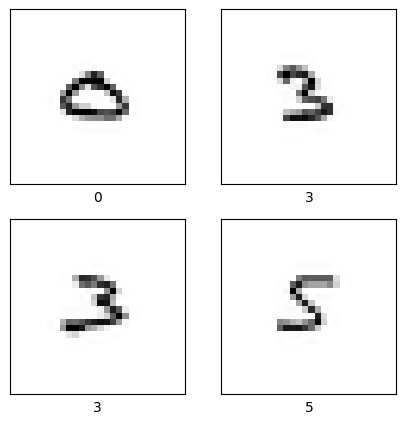
\includegraphics[width=\linewidth]{Bilder/emnist_client1.png}
        \caption{Client \texttt{f0599\_04} has 105 images in total}
    \end{subfigure}
    \hfill
    \begin{subfigure}{0.4\textwidth}
    		\centering        
        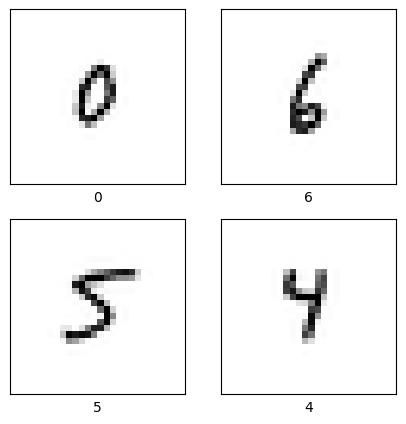
\includegraphics[width=\linewidth]{Bilder/emnist_client2.png}
        \caption{Client \texttt{f0654\_02} has 105 images in total}
    \end{subfigure}
    	\caption{Handwritten digits of different clients showing the difference in data distribution}
    \label{fig:mnist-digits}
\end{figure}

\subsection{SVHN}

Der Street View House Numbers Datensatz \parencite{netzer:2011} ist ähnlich wie MNIST ein Datensatz um Ziffern zu erkennen. Allerdings liegen sie in diesem Fall als Bilder von Hausnummern aus Google Street View vor. Von dem Datensatz gibt es zwei Versionen: die erste enthält ganze Bilder und Bounding Boxes für jede Ziffer, die zweite enthält bereits gecroppte 32x32 Pixel große Bilder mit einzelnen Ziffern.

Für meine Arbeit habe ich die zweite Version genutzt. 

\subsection{CIFAR100}
